\let\negmedspace\undefined
\let\negthickspace\undefined
\documentclass[journal,12pt,onecolumn]{IEEEtran}
\usepackage{cite}
\usepackage{amsmath,amssymb,amsfonts,amsthm}
\usepackage{algorithmic}
\usepackage{graphicx}
\graphicspath{{./figs/}}
\usepackage{textcomp}
\usepackage{xcolor}
\usepackage{txfonts}
\usepackage{listings}
\usepackage{enumitem}
\usepackage{mathtools}
\usepackage{gensymb}
\usepackage{comment}
\usepackage{caption}
\usepackage[breaklinks=true]{hyperref}
\usepackage{tkz-euclide} 
\usepackage{listings}
\usepackage{gvv}                                        
%\def\inputGnumericTable{}                                 
\usepackage[latin1]{inputenc}     
\usepackage{xparse}
\usepackage{color}                                            
\usepackage{array}                                            
\usepackage{longtable}                                       
\usepackage{calc}                                             
\usepackage{multirow}
\usepackage{multicol}
\usepackage{hhline}                                           
\usepackage{ifthen}                                           
\usepackage{lscape}
\usepackage{tabularx}
\usepackage{array}
\usepackage{float}
%\newtheorem{theorem}{Theorem}[section]
%\newtheorem{theorem}{Theorem}[section]
%\newtheorem{problem}{Problem}
%\newtheorem{proposition}{Proposition}[section]
%\newtheorem{lemma}{Lemma}[section]
%\newtheorem{corollary}[theorem]{Corollary}
%\newtheorem{example}{Example}[section]
%\newtheorem{definition}[problem]{Definition}

\begin{document}

\title{4.13.25}
\author{EE25BTECH11020 - Darsh Pankaj Gajare}
% \maketitle
% \newpage
% \bigskip
%\begin{document}
{\let\newpage\relax\maketitle}
%\renewcommand{\thefigure}{\theenumi}
%\renewcommand{\thetable}{\theenumi}
Question:\\
Two sides of a rhombus are along the lines, $x - y + 1 = 0$ and $7x - y - 5 = 0$. If its diagonals intersect at $\brak{-1, -2}$, then which one of the following is a vertex of this rhombus?
\begin{enumerate}
		\begin{multicols}{4}
		\item $\brak{\frac{1}{3},-\frac{8}{3}}$
		\item $\brak{-\frac{10}{3},-\frac{7}{3}}$
		\item $\brak{-3,-9}$
		\item $\brak{-3,-8}$
		\end{multicols}
\end{enumerate}
\solution
\begin{table}[H]
	\centering
	\caption{}
	\begin{tabular}{|c|c|}
\hline
\textbf{Name} & \textbf{Value} \\
\hline
Circle & $\vec{x}^\top\vec{x} - a^2 = 0$ \\
\hline
Line & $\vec{x} = \myvec{\tfrac{a}{\sqrt{2}} \\ 0} + \kappa\myvec{0 \\ 1}$ \\
\hline
\end{tabular}

	\label{}
\end{table}
\begin{align}
A\vec{V_A} &= b, \quad 
A=\myvec{1 & -1\\ 7 & -1},\ 
b=\myvec{-1\\ 5} \\ 
\augvec{2}{1}{1 & -1 & -1\\ 7 & -1 & 5} 
&\xrightarrow{R_2-7R_1} 
\augvec{2}{1}{1 & -1 & -1\\ 0 & 6 & 12} \\ 
\vec{V_A} &= \myvec{1\\2} 
\end{align}

\begin{align}
\vec{V_C} &= 2\vec{O}-\vec{V_A}
=2\myvec{-1\\-2}-\myvec{1\\2}
=\myvec{-3\\-6}
\end{align}

\begin{align}
k &= -\vec{n_1}^T\vec{V_C}=-3, \quad
m=-\vec{n_2}^T\vec{V_C}=15
\end{align}

\begin{align}
\augvec{2}{1}{1 & -1 & 3\\ 7 & -1 & 5}
&\xrightarrow{R_2-7R_1}
\augvec{2}{1}{1 & -1 & 3\\ 0 & 6 & -16} \\ 
\vec{V} = \myvec{\frac{1}{3}\\ -\frac{8}{3}} \\ 
\end{align}
Plot using C libraries:
\begin{figure}[H]
	\centering
	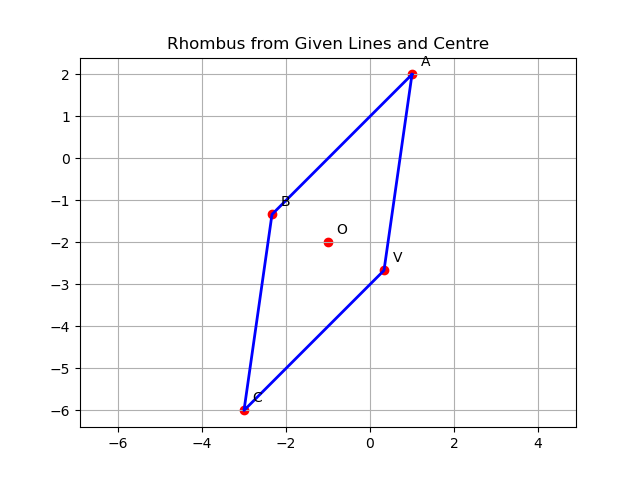
\includegraphics[scale=0.5]{img1}
	\caption*{}
	\label{img1}
\end{figure}
Plot using Python:
\begin{figure}[H]
	\centering
	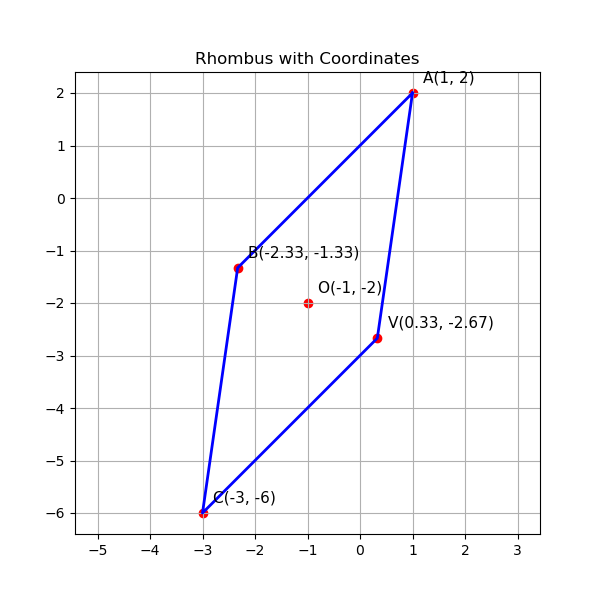
\includegraphics[scale=0.5]{img2}
	\caption*{}
	\label{img2}
\end{figure}
\end{document}

